\chapter{在苦難中忠心作見證（10:1-11:19）}

上一章我們讀了第一號到第六號，現在該輪到第七號了吧？然而，啟示錄在第七號之前，插入了兩段故事：「約翰再多說預言」和「兩位見證人」，然後才進入第七號。為什麼要插入這兩個故事呢？這兩段經文都讓我們看見，在神的審判進行之時，祂的子民仍然肩負為祂作見證的使命。即使面對苦難與逼迫，他們仍要忠心見證神的話語，直到基督的國度完全顯明。

\section{約翰再多說預言}

\begin{ScriptureBox}

\item[10:1] 我又看見另有一位大力的天使、從天降下、披著雲彩、頭上有虹．臉面像日頭、兩腳像火柱．

\item[10:2] 他手裡拿著小書卷是展開的．他右腳踏海、左腳踏地．

\item[10:3] 大聲呼喊、好像獅子吼叫、呼喊完了、就有七雷發聲。

\item[10:4] 七雷發聲之後、我正要寫出來、就聽見從天上有聲音說、七雷所說的你要封上、不可寫出來。

\item[10:5] 我所看見的那踏海踏地的天使、向天舉起右手來、

\item[10:6] 指著那創造天和天上之物、地和地上之物、海和海中之物、直活到永永遠遠的、起誓說、不再有時日了．〔或作不再耽延了〕

\item[10:7] 但在第七位天使吹號發聲的時候、　神的奧秘、就成全了、正如　神所傳給他僕人眾先知的佳音。

\item[10:8] 我先前從天上所聽見的那聲音、又吩咐我說、你去把那踏海踏地之天使手中展開的小書卷取過來．

\item[10:9] 我就走到天使那裡、對他說、請你把小書卷給我．他對我說、你拿著喫盡了、便叫你肚子發苦、然而在你口中要甜如蜜。

\item[10:10] 我從天使手中把小書卷接過來、喫盡了．在我口中果然甜如蜜．喫了以後、肚子覺得發苦了。

\item[10:11] 天使〔原文作他們〕對我說、你必指著多民多國多方多王再說預言。

\end{ScriptureBox}

\begin{figure}[htbp]
    \centering
    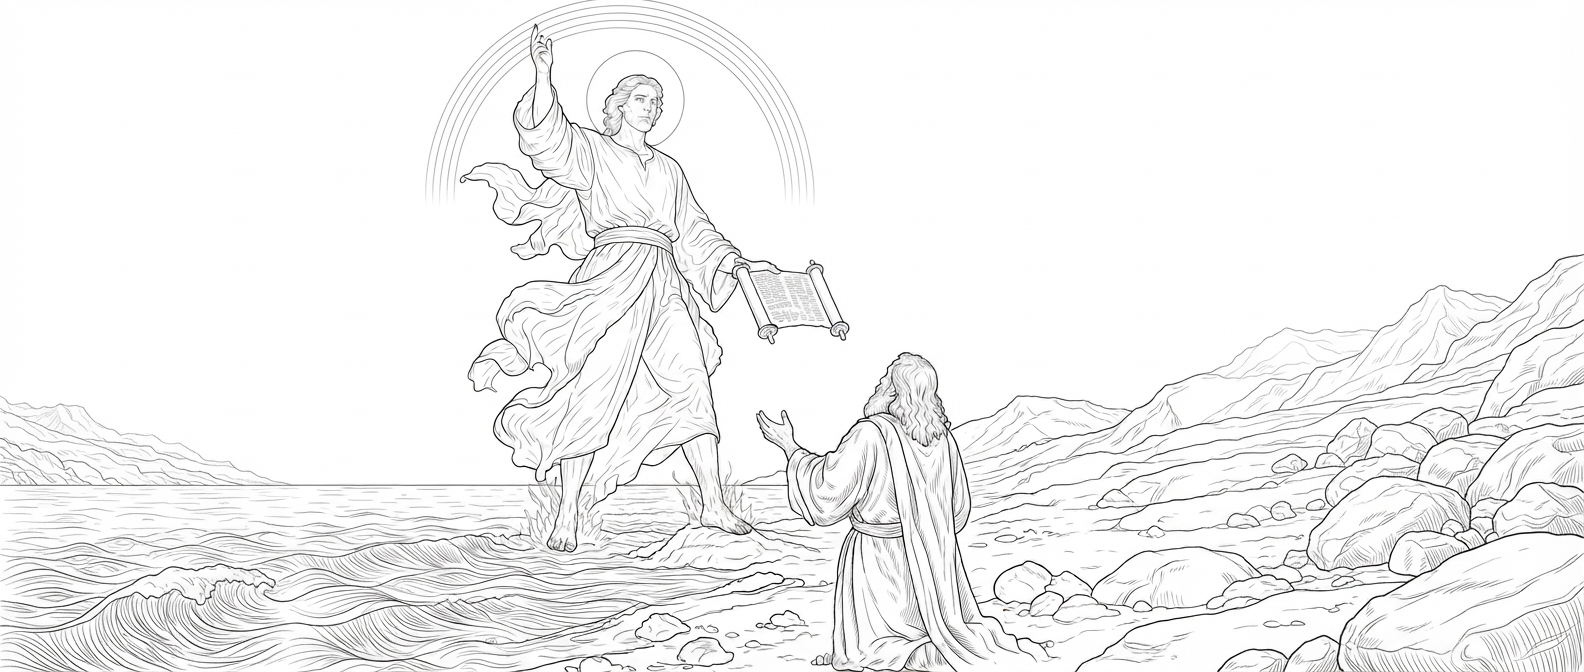
\includegraphics[
    width=1\textwidth, 
    trim=200 0 200 0, 
    clip]{images/small_scroll2.jpg}
\end{figure}

神的話在口中甜如蜜，因為它帶來神的真理並帶來安慰。神的話使得約翰腹中發苦，因為忠心傳揚這真理，也意味著面對審判、苦難與逼迫。

約翰正要寫下所聽見的內容時，卻有聲音從天上吩咐他「不可寫出來。」這表明神決定哪些事情可以讓約翰知道，哪些事情仍然隱藏。
申命記29:29說：「隱祕的事是屬耶和華我們神的；惟有明顯的事是永遠屬我們和我們子孫的。」
我們信仰的重點不在於知道每一個末世細節，而在於相信神掌管歷史，並忠心領受祂已經啟示的真理。
這裡有一個重要的屬靈功課，就是我們要以謙卑的心面對尚未顯明的事，專注遵行神已經向我們啟示的話語。


\section{兩個見證人}

\begin{ScriptureBox}

\item[11:1] 有一根葦子賜給我、當作量度的杖．且有話說、起來、將　神的殿、和祭壇、並在殿中禮拜的人、都量一量。

\item[11:2] 只是殿外的院子、要留下不用量．因為這是給了外邦人的．他們要踐踏聖城四十二個月。

\item[11:3] 我要使我那兩個見證人、穿著毛衣、傳道一千二百六十天。

\item[11:4] 他們就是那兩棵橄欖樹、兩個燈臺、立在世界之主面前的。

\item[11:5] 若有人想要害他們就有火從他們口中出來、燒滅仇敵．凡想要害他們的、都必這樣被殺。

\item[11:6] 這二人有權柄、在他們傳道的日子叫天閉塞不下雨．又有權柄、叫水變為血．並且能隨時隨意用各樣的災殃攻擊世界。

\item[11:7] 他們作完見證的時候、那從無底坑裡上來的獸、必與他們交戰、並且得勝、把他們殺了。

\item[11:8] 他們的屍首就倒在大城裡的街上．這城按著靈意叫所多瑪、又叫埃及、就是他們的主釘十字架之處。

\item[11:9] 從各民各族各方各國中、有人觀看他們的屍首三天半、又不許把屍首放在墳墓裡。

\item[11:10] 住在地上的人、就為他們歡喜快樂、互相餽送禮物．因這兩位先知曾叫住在地上的人受痛苦。

\item[11:11] 過了這三天半、有生氣從　神那裡進入他們裡面、他們就站起來、看見他們的人甚是害怕。

\item[11:12] 兩位先知聽見有大聲音從天上來、對他們說、上到這裡來。他們就駕著雲上了天．他們的仇敵也看見了。

\item[11:13] 正在那時候、地大震動、城就倒塌了十分之一．因地震而死的有七千人．其餘的都恐懼、歸榮耀給天上的　神。

\end{ScriptureBox}

\subsection{量度神的殿和聖城被踐踏}

在聖經的異象中，我們會讀到量度聖殿。例如，以西結書40–48章量度聖殿，撒迦利亞書2:1–5也記載量度耶路撒冷的異象。
那象徵神對祂所量度之物的認定、分別或保守。
殿外的院子不量，因為它被交給外邦人，聖城也要被踐踏四十二個月。神的子民雖然屬於神，卻仍可能在地上遭受逼迫。

多久呢？聖經在不同的異象中，提到幾個彼此呼應的時間：「四十二個月」（啟示錄 11:2）、「一千二百六十天」（啟示錄 11:3），以及「一載、二載、半載」（1+2+$\frac{1}{2}=3\frac{1}{2}$）（啟示錄 12:14）。按照一年十二個月、每月三十天計算，這些時間都相當於三年半。對於這三年半應如何理解，不同的解經觀點有不同的解釋與應用。相關的討論，我放在「附錄：大災難多久？但以理書的七十個七」。無論採取哪一種解經觀點，此三年半都代表一段有限的受苦時期，也就是說敵對神的勢力不是無限期的。


\begin{figure}[htbp]
    \centering
    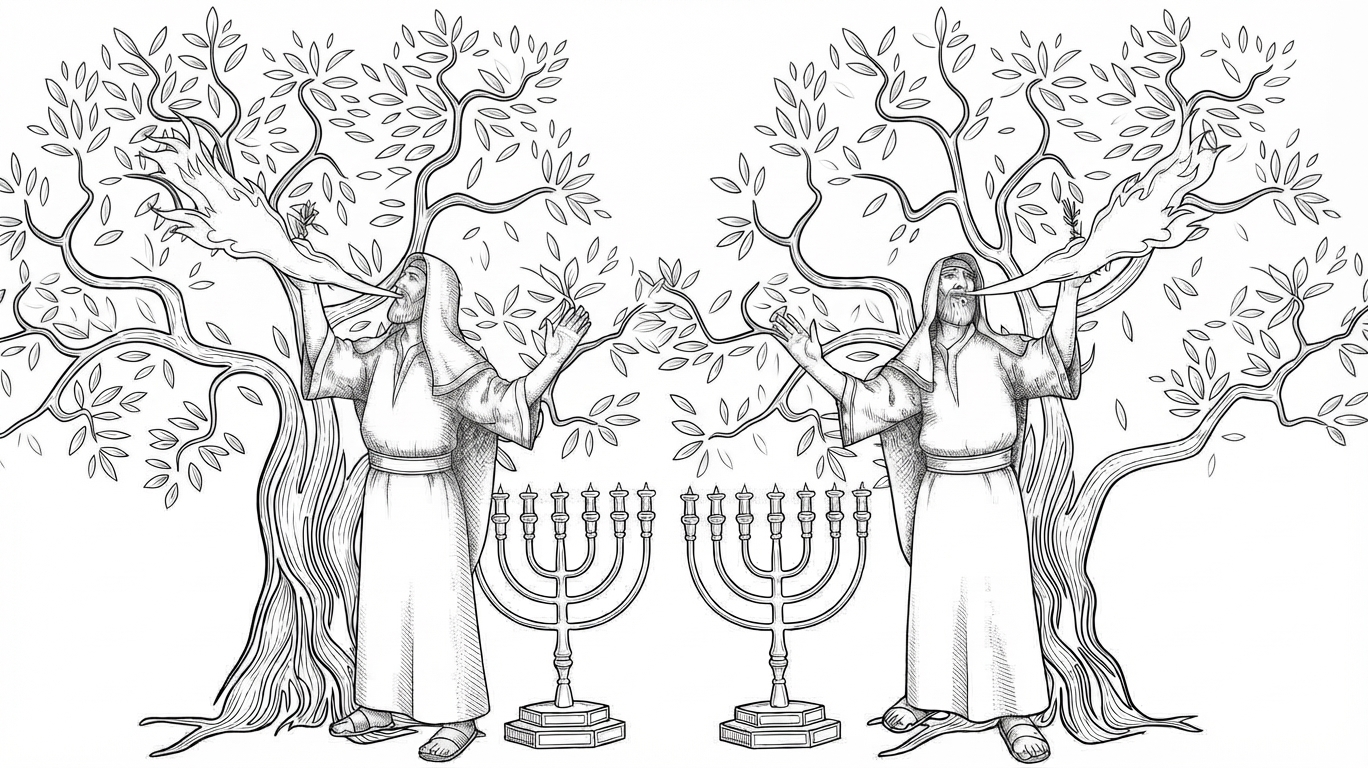
\includegraphics[
    width=1\textwidth, 
    trim=0 0 0 0, 
    clip]{images/two_witnesses.jpg}
\end{figure}


\subsection{兩位見證人是誰？}

此處約翰的預言有大量使用舊約的背景。所以我用表\ref{tab:rev11-ot-background-zh}來了解這些背景以及意涵。


{
\small
\renewcommand{\arraystretch}{1}
%\setlength{\LTpre}{0pt}
%\setlength{\LTpost}{0pt}

\begin{longtable}{
    @{}
    p{0.24\textwidth} |
    p{0.30\textwidth}
    p{0.36\textwidth}
    @{}
}
\caption{啟示錄11章的舊約背景}
\label{tab:rev11-ot-background-zh} \\
\hline 
啟示錄 11 & 舊約背景 & 意涵 \\
\hline
\endfirsthead

啟示錄 11 & 舊約背景 & 意涵 \\
\hline
\endhead

兩個見證人
& 申命記 19:15
& 兩三個見證人的原則 \\

兩棵橄欖樹
& 撒迦利亞 4:1--14
& 橄欖樹、燈臺 \\

兩個燈臺
& 撒迦利亞 4 章；啟示錄 1:20
& 見證與神的子民 \\

火從口中出來
& 耶利米書 5:14
& 神話語審判能力 \\

天閉塞
& 列王紀上 17:1
& 以利亞 \\

水變為血
& 出埃及記7:14-25
& 摩西 \\

各樣災殃
& 出埃及記
& 出埃及記的災禍 \\

無底坑的獸
& 但以理書7章
& 敵對神的政權 \\

所多瑪、埃及
& 創世記、出埃及記
& 敗壞與壓迫神子民的世界 \\

復活
& 以西結書 37 章
& 神使死人得生命 \\

駕雲上天
& 但以理書 7:13；列王紀下 2 章
& 神的榮耀與升天 \\
\hline
\end{longtable}
}

有了以上的舊約背景，我們才能了解不同神學家所提出的，關於兩位見證人是誰的假設。我列表\ref{tab:two-witnesses-zh}如下。

{
\small
\renewcommand{\arraystretch}{1}

\begin{longtable}{
    @{}
    p{0.3\textwidth} |
    p{0.66\textwidth}
    @{}
}
\caption{兩個見證人是誰？}
\label{tab:two-witnesses-zh} \\
\hline 
人物 & 主要依據  \\
\hline
\endfirsthead

兩個見證人是誰？ & 主要依據 \\

\endhead
以諾、以利亞
& 二人都沒有經歷死亡而被神接去 \\

摩西、以利亞
& 火、旱災、降災等神蹟呼應以利亞與摩西；二人一同出現在登山變像。\footnote{Grant R. Osborne、John MacArthur} \\

神將在末世興起的兩位實際人物
& 其具體的傳道、受死、復活與升天。\footnote{John MacArthur 等前千禧年派解經家} \\

忠心的教會和神的子民
& 橄欖樹、燈臺象徵教會。\footnote{G. K. Beale、Craig R. Koester} \\
\hline
\end{longtable}
}

\subsection{第二、三樣災禍包括什麼？}

\begin{ScriptureBox}
\item[11:14] 第二樣災禍過去．第三樣災禍快到了。
\end{ScriptureBox}

第二樣災禍包括第六號所帶來的審判，以及兩位見證人的異象。
第三樣災禍是由第七號吹響開始的。見圖\ref{fig:trumpets_woes}。

\section{第七號響}


\begin{ScriptureBox}

\item[11:15] 第七位天使吹號、天上就有大聲音說、世上的國、成了我主和主基督的國．他要作王、直到永永遠遠。

\item[11:16] 在　神面前、坐在自己位上的二十四位長老、就面伏於地敬拜　神、

\item[11:17] 說、昔在今在的主　神、全能者阿、我們感謝你、因你執掌大權作王了。

\item[11:18] 外邦發怒、你的忿怒也臨到了．審判死人的時候也到了．你的僕人眾先知、和眾聖徒、凡敬畏你名的人連大帶小得賞賜的時候也到了．你敗壞那些敗壞世界之人的時候也就到了。

\item[11:19] 當時　神天上的殿開了．在他殿中現出他的約櫃．隨後有閃電、聲音、雷轟、地震、大雹。

\end{ScriptureBox}

第七號吹響，天上首先宣告的不是另一場災難，而是基督必然掌權的事實。
這裡宣告，神的忿怒已經臨到，審判的時刻已經到了。這不再只是「三分之一」所代表的局部災難，而是神對邪惡施行完全的審判、追討罪惡的時刻。下一章，我們將進一步看見這場爭戰的屬靈本質，以及敵對神的勢力如何走向敗亡。

\section*{小組討論題}

\begin{enumerate}
\item 為什麼神的話會同時「甜如蜜」又「發苦」？
\item 兩個見證人被獸殺害，而且世上的人因他們死亡而歡喜。今天我們是否也會因為害怕人的反應，而不敢忠於基督？
\item 如果神今天要你在自己的家庭、教會、職場或朋友圈中作一個忠心的見證人，你覺得祂可能要你持守什麼、改變什麼，或勇敢說出什麼？
\end{enumerate}

